\documentclass[border=0pt]{standalone}
\usepackage[T1]{fontenc}
\usepackage{helvet}
\renewcommand{\familydefault}{\sfdefault}
\usepackage{amsmath,amssymb}
\usepackage{tikz}
\usetikzlibrary{arrows.meta,positioning}
\definecolor{ink}{HTML}{262B30}
\definecolor{callred}{HTML}{C44C3C}
\definecolor{emitblue}{HTML}{356D96}
\definecolor{edgequiet}{HTML}{8E979E}
\definecolor{holdstroke}{HTML}{C5CCD2}
\tikzset{
  title/.style={font=\sffamily\bfseries\fontsize{8.7}{10}\selectfont, text=ink, inner sep=0pt, anchor=base},
  digit/.style={font=\sffamily\fontsize{7.5}{8.6}\selectfont, text=ink, inner sep=0pt},
  digitw/.style={font=\sffamily\fontsize{7.5}{8.6}\selectfont, text=white, inner sep=0pt},
  runlab/.style={font=\sffamily\fontsize{7.2}{8.4}\selectfont, text=ink, inner sep=0pt, anchor=base},
  annot/.style={font=\sffamily\fontsize{7.2}{8.4}\selectfont, text=callred, inner sep=0pt},
  pi/.style={font=\sffamily\fontsize{7.2}{8.4}\selectfont, text=emitblue, inner sep=0pt, anchor=west},
  legend/.style={font=\sffamily\fontsize{7.3}{8.6}\selectfont, text=ink, inner sep=0pt, anchor=west},
  stored/.style={draw=ink, line width=0.9pt, fill=white, rounded corners=7.15pt},
  unread/.style={draw=holdstroke, line width=0.8pt, fill=white, rounded corners=7.15pt},
  incall/.style={draw=callred, line width=1.15pt, fill=white, rounded corners=7.15pt},
  emitted/.style={draw=emitblue, line width=0.95pt, fill=emitblue, rounded corners=7.15pt},
  tree/.style={draw=edgequiet, line width=0.75pt, line cap=round},
  pathedge/.style={draw=ink, line width=1.65pt, line cap=round},
  ptr/.style={draw=ink, line width=1.15pt, line cap=round,
              -{Stealth[length=1.45mm,width=1.15mm,inset=0.2pt]}},
  win/.style={draw=emitblue, line width=1.15pt, line cap=round,
              -{Stealth[length=1.45mm,width=1.15mm,inset=0.2pt]}},
  seq/.style={draw=edgequiet, line width=0.8pt, line cap=round,
              -{Stealth[length=1.25mm,width=1.05mm]}},
  lead/.style={draw=callred, line width=0.65pt, line cap=round,
               -{Stealth[length=1.05mm,width=0.8mm,inset=0.15pt]}},
  legsw/.style={line width=0.7pt, rounded corners=1.15pt},
}
\begin{document}
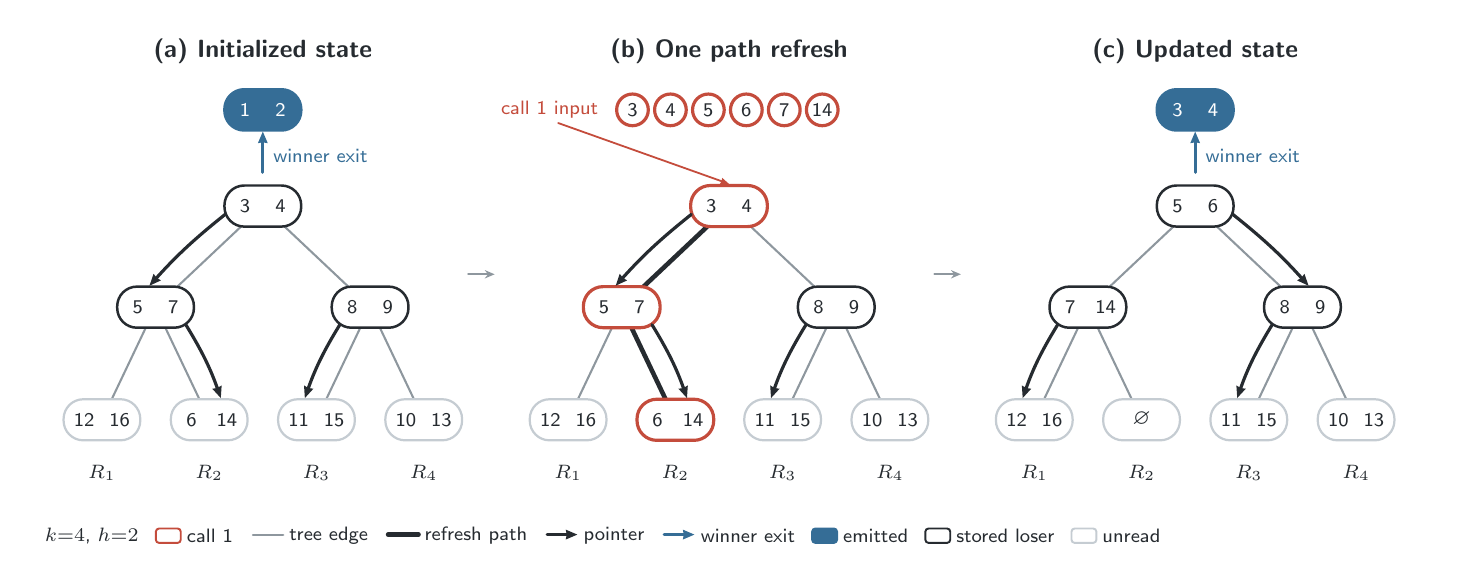
\begin{tikzpicture}[x=1bp,y=1bp]
\useasboundingbox (0,0) rectangle (504.960,187.920);
  \node[title] at (84.655,177.266) {(a) Initialized state};
  \node[title] at (252.480,177.266) {(b) One path refresh};
  \node[title] at (420.305,177.266) {(c) Updated state};
  \draw[tree] (76.686,116.190) -- (54.009,94.813);
  \draw[tree] (92.624,116.190) -- (115.301,94.813);
  \draw[tree] (42.371,79.596) -- (30.403,54.464);
  \draw[tree] (49.710,79.596) -- (61.678,54.464);
  \draw[tree] (119.600,79.596) -- (107.632,54.464);
  \draw[tree] (126.939,79.596) -- (138.907,54.464);
  \draw[stored] (70.843,116.303) rectangle (98.467,131.100);
  \draw[stored] (32.228,79.903) rectangle (59.853,94.700);
  \draw[stored] (109.458,79.903) rectangle (137.082,94.700);
  \node[digit] at (78.269,123.702) {3};
  \node[digit] at (91.041,123.702) {4};
  \node[digit] at (39.654,87.301) {5};
  \node[digit] at (52.427,87.301) {7};
  \node[digit] at (116.883,87.301) {8};
  \node[digit] at (129.656,87.301) {9};
  \draw[unread] (12.921,39.360) rectangle (40.545,54.156);
  \node[digit] at (20.347,46.758) {12};
  \node[digit] at (33.119,46.758) {16};
  \node[runlab] at (26.733,25.747) {$R_1$};
  \draw[unread] (51.536,39.360) rectangle (79.160,54.156);
  \node[digit] at (58.962,46.758) {6};
  \node[digit] at (71.734,46.758) {14};
  \node[runlab] at (65.348,25.747) {$R_2$};
  \draw[unread] (90.150,39.360) rectangle (117.774,54.156);
  \node[digit] at (97.576,46.758) {11};
  \node[digit] at (110.349,46.758) {15};
  \node[runlab] at (103.962,25.747) {$R_3$};
  \draw[unread] (128.765,39.360) rectangle (156.389,54.156);
  \node[digit] at (136.191,46.758) {10};
  \node[digit] at (148.963,46.758) {13};
  \node[runlab] at (142.577,25.747) {$R_4$};
  \draw[emitted] (70.843,150.928) rectangle (98.467,165.725);
  \node[digitw] at (78.269,158.326) {1};
  \node[digitw] at (91.041,158.326) {2};
  \draw[win] (84.655,135.835) -- (84.655,150.573);
  \node[pi] at (88.219,141.754) {winner exit};
  \draw[ptr] (71.092,120.694) .. controls (59.717,111.601) and (53.539,105.777) .. (43.797,94.964);
  \draw[ptr] (56.949,80.963) .. controls (62.778,71.484) and (65.868,64.997) .. (69.550,54.504);
  \draw[ptr] (112.361,80.963) .. controls (106.532,71.484) and (103.443,64.997) .. (99.761,54.504);
  \draw[tree] (260.449,116.190) -- (283.126,94.813);
  \draw[tree] (210.196,79.596) -- (198.228,54.464);
  \draw[tree] (287.425,79.596) -- (275.457,54.464);
  \draw[tree] (294.764,79.596) -- (306.732,54.464);
  \draw[pathedge] (244.511,116.190) -- (221.834,94.813);
  \draw[pathedge] (217.535,79.596) -- (229.503,54.464);
  \draw[incall] (238.668,116.303) rectangle (266.292,131.100);
  \draw[incall] (200.053,79.903) rectangle (227.678,94.700);
  \draw[stored] (277.282,79.903) rectangle (304.907,94.700);
  \node[digit] at (246.094,123.702) {3};
  \node[digit] at (258.866,123.702) {4};
  \node[digit] at (207.479,87.301) {5};
  \node[digit] at (220.252,87.301) {7};
  \node[digit] at (284.708,87.301) {8};
  \node[digit] at (297.481,87.301) {9};
  \draw[unread] (180.746,39.360) rectangle (208.370,54.156);
  \node[digit] at (188.172,46.758) {12};
  \node[digit] at (200.944,46.758) {16};
  \node[runlab] at (194.558,25.747) {$R_1$};
  \draw[incall] (219.361,39.360) rectangle (246.985,54.156);
  \node[digit] at (226.786,46.758) {6};
  \node[digit] at (239.559,46.758) {14};
  \node[runlab] at (233.173,25.747) {$R_2$};
  \draw[unread] (257.975,39.360) rectangle (285.599,54.156);
  \node[digit] at (265.401,46.758) {11};
  \node[digit] at (278.174,46.758) {15};
  \node[runlab] at (271.787,25.747) {$R_3$};
  \draw[unread] (296.590,39.360) rectangle (324.214,54.156);
  \node[digit] at (304.016,46.758) {10};
  \node[digit] at (316.788,46.758) {13};
  \node[runlab] at (310.402,25.747) {$R_4$};
  \draw[ptr] (238.917,120.694) .. controls (227.542,111.601) and (221.364,105.777) .. (211.622,94.964);
  \draw[ptr] (224.774,80.963) .. controls (230.603,71.484) and (233.692,64.997) .. (237.374,54.504);
  \draw[ptr] (280.186,80.963) .. controls (274.357,71.484) and (271.268,64.997) .. (267.586,54.504);
  \node[annot, anchor=west] (callin) at (170.201,158.326) {call 1 input};
  \draw[incall] (217.727,158.326) circle (5.70bp);
  \node[digit] at (217.727,158.326) {3};
  \draw[incall] (231.390,158.326) circle (5.70bp);
  \node[digit] at (231.390,158.326) {4};
  \draw[incall] (245.054,158.326) circle (5.70bp);
  \node[digit] at (245.054,158.326) {5};
  \draw[incall] (258.718,158.326) circle (5.70bp);
  \node[digit] at (258.718,158.326) {6};
  \draw[incall] (272.381,158.326) circle (5.70bp);
  \node[digit] at (272.381,158.326) {7};
  \draw[incall] (286.045,158.326) circle (5.70bp);
  \node[digit] at (286.045,158.326) {14};
  \draw[lead] (190.994,153.591) -- (252.480,131.692);
  \draw[tree] (412.336,116.190) -- (389.659,94.813);
  \draw[tree] (428.274,116.190) -- (450.951,94.813);
  \draw[tree] (378.021,79.596) -- (366.053,54.464);
  \draw[tree] (385.360,79.596) -- (397.328,54.464);
  \draw[tree] (455.250,79.596) -- (443.282,54.464);
  \draw[tree] (462.589,79.596) -- (474.557,54.464);
  \draw[stored] (406.493,116.303) rectangle (434.117,131.100);
  \draw[stored] (367.878,79.903) rectangle (395.502,94.700);
  \draw[stored] (445.107,79.903) rectangle (472.732,94.700);
  \node[digit] at (413.919,123.702) {5};
  \node[digit] at (426.691,123.702) {6};
  \node[digit] at (375.304,87.301) {7};
  \node[digit] at (388.077,87.301) {14};
  \node[digit] at (452.533,87.301) {8};
  \node[digit] at (465.306,87.301) {9};
  \draw[unread] (348.571,39.360) rectangle (376.195,54.156);
  \node[digit] at (355.997,46.758) {12};
  \node[digit] at (368.769,46.758) {16};
  \node[runlab] at (362.383,25.747) {$R_1$};
  \draw[unread] (387.185,39.360) rectangle (414.810,54.156);
  \node[digit] at (400.998,46.758) {$\varnothing$};
  \node[runlab] at (400.998,25.747) {$R_2$};
  \draw[unread] (425.800,39.360) rectangle (453.424,54.156);
  \node[digit] at (433.226,46.758) {11};
  \node[digit] at (445.998,46.758) {15};
  \node[runlab] at (439.612,25.747) {$R_3$};
  \draw[unread] (464.415,39.360) rectangle (492.039,54.156);
  \node[digit] at (471.841,46.758) {10};
  \node[digit] at (484.613,46.758) {13};
  \node[runlab] at (478.227,25.747) {$R_4$};
  \draw[emitted] (406.493,150.928) rectangle (434.117,165.725);
  \node[digitw] at (413.919,158.326) {3};
  \node[digitw] at (426.691,158.326) {4};
  \draw[win] (420.305,135.835) -- (420.305,150.573);
  \node[pi] at (423.869,141.754) {winner exit};
  \draw[ptr] (433.868,120.694) .. controls (445.243,111.601) and (451.421,105.777) .. (461.163,94.964);
  \draw[ptr] (370.781,80.963) .. controls (364.952,71.484) and (361.863,64.997) .. (358.181,54.504);
  \draw[ptr] (448.011,80.963) .. controls (442.182,71.484) and (439.092,64.997) .. (435.410,54.504);
  \draw[seq] (158.617,99.139) -- (168.122,99.139);
  \draw[seq] (326.442,99.139) -- (335.947,99.139);
  \node[legend] (L0) at (6bp,5.031) {$k{=}4$, $h{=}2$};
  \draw[legsw, draw=callred, fill=white] ([xshift=6pt,yshift=-2.6pt]L0.east) rectangle ++(9pt,5.2pt);
  \node[legend, anchor=west] (L1) at ([xshift=17pt]L0.east) {call 1};
  \draw[tree] ([xshift=7pt,yshift=0.4pt]L1.east) -- ++(11pt,0);
  \node[legend, anchor=west] (L2) at ([xshift=20pt]L1.east) {tree edge};
  \draw[pathedge] ([xshift=7pt,yshift=0.4pt]L2.east) -- ++(11pt,0);
  \node[legend, anchor=west] (L3) at ([xshift=20pt]L2.east) {refresh path};
  \draw[ptr] ([xshift=7pt,yshift=0.4pt]L3.east) -- ++(11pt,0);
  \node[legend, anchor=west] (L4) at ([xshift=20pt]L3.east) {pointer};
  \draw[win] ([xshift=7pt,yshift=0.4pt]L4.east) -- ++(11pt,0);
  \node[legend, anchor=west] (L5) at ([xshift=20pt]L4.east) {winner exit};
  \draw[legsw, draw=emitblue, fill=emitblue] ([xshift=6pt,yshift=-2.6pt]L5.east) rectangle ++(9pt,5.2pt);
  \node[legend, anchor=west] (L6) at ([xshift=17pt]L5.east) {emitted};
  \draw[legsw, draw=ink, fill=white] ([xshift=6pt,yshift=-2.6pt]L6.east) rectangle ++(9pt,5.2pt);
  \node[legend, anchor=west] (L7) at ([xshift=17pt]L6.east) {stored loser};
  \draw[legsw, draw=holdstroke, fill=white] ([xshift=6pt,yshift=-2.6pt]L7.east) rectangle ++(9pt,5.2pt);
  \node[legend, anchor=west] (L8) at ([xshift=17pt]L7.east) {unread};
\end{tikzpicture}
\end{document}
